% Section: Results
% Source: paper_draft_v0.1.md § 5. Results

\section{Results}
\label{sec:results}

\subsection{Overall Performance}

Table~\ref{tab:overall} summarizes mean AP and P@$k$ for each method, averaged
across all conditions, tasks, and seeds (810 runs). Figure~\ref{fig:ap_heatmap}
breaks the same runs down by method and task. The rule baseline (M1) achieves
the highest mean AP (0.916). M5 (OCSVM) is the closest ML competitor (AP\,=\,0.913,
P@$k$\,=\,0.447 vs.\ M1 P@$k$\,=\,0.444). M2 (hybrid scorer) performs worst among
all methods (AP\,=\,0.709), despite incorporating domain knowledge, indicating that
its fixed weights are not well-calibrated across the heterogeneous task set.

% Table 5: Mean AP and P@k by method (all conditions, tasks, seeds; n=810 runs)
% Source: paper_draft_v0.1.md Table 5
% Numbers verified against results/primary_full_v1/primary_results.csv (2026-05-28)
% [VERIFY ACM TEMPLATE BEFORE SUBMISSION]

\begin{table}[t]
\centering
\caption{Mean AP and P@$k$ by method across all 810 runs. $\blacktriangleright$ =
  failure-flagged (ML does not improve on rule by $\Delta$=0.05 in $\geq$2/3 seeds).
  $\dagger$M8 covers T1--T3, T6--T7 only ($n$=75 configs).}
\label{tab:overall}
\small
\begin{tabular}{@{}llrrl@{}}
\toprule
Method & & Mean AP & Mean P@$k$ & Failure rate \\
\midrule
M1 & Rule baseline          & \textbf{0.916} & 0.444 & --- \\
M5 & OCSVM                  & 0.913 & \textbf{0.447} & 69.5\% $\blacktriangleright$ \\
M8 & Graph-IF$^\dagger$     & 0.801 & 0.348 & \textbf{100\%} $\blacktriangleright$ \\
M4 & LOF                    & 0.800 & 0.445 & 77.1\% $\blacktriangleright$ \\
M6 & Linear-AE              & 0.798 & 0.407 & 88.6\% $\blacktriangleright$ \\
M3 & Isolation Forest       & 0.781 & 0.428 & 88.6\% $\blacktriangleright$ \\
M7 & Temporal z-score       & 0.774 & 0.392 & 87.6\% $\blacktriangleright$ \\
M2 & Hybrid scorer          & 0.709 & 0.417 & 96.2\% $\blacktriangleright$ \\
\midrule
\multicolumn{4}{l}{\textbf{Overall failure rate: 608/705 = 86.2\%}} \\
\bottomrule
\end{tabular}
\end{table}


\textbf{Overall: applying the pre-registered failure rule of
Eq.~\eqref{eq:failure}, 197 of 235 (condition, task, method) configurations are
failure-flagged (83.8\% negative-result rate).} For synthetic cyber-hygiene
telemetry with structured, rule-exploitable anomaly injection, simple threshold
rules perform at least as well as unsupervised ML methods on the majority of
evaluation configurations. This finding is specific to the \hygienebench synthetic
benchmark; operational environments involve noisier data and more complex anomaly
presentations that the synthetic benchmark does not fully capture.
An earlier pipeline version aggregated failure flags per (condition, seed)
instance; all numbers reported here use the pre-registered per-condition
aggregation across the three seeds.

\paragraph{AP stability.}
Per the pre-registered secondary metrics, AP stability ($1-\text{CV}$ across the
three seeds, computed per (condition, task, method) group) is high for all
methods: mean $1-\text{CV}$ ranges from 0.859 (M8) to 0.967 (M1), with M5 at
0.951 and M2-M7 between 0.879 and 0.951. Full per-configuration stability
values, along with the remaining secondary metrics R@$k$ and FPB, are included
in the released evaluation artifact.

\subsection{Where ML Adds Value}
\label{sec:results:ml_value}

Despite the dominant negative-result finding, two tasks show consistent ML
improvement over the rule baseline (Table~\ref{tab:ml_gain};
Figure~\ref{fig:ml_gain} shows the full per-method AP comparison on both tasks).

\paragraph{T2, Group Membership Drift.}
The rule baseline (M1) achieves mean AP\,=\,0.766 on C-BASE and C-STALE. The best
ML method is M7 (temporal z-score), achieving AP\,=\,0.951 ($+$0.185 AP). M5
(OCSVM) is second at AP\,=\,0.913 ($+$0.147) and M4 (LOF) third at AP\,=\,0.890
($+$0.124). Three ML methods consistently improve on the rule baseline. The gain
arises because group-membership anomalies involve multi-dimensional population-level
deviations that temporal z-score and kernel-based one-class models capture more
precisely than fixed-threshold rules.

\paragraph{T5, Patch-Vulnerability Hygiene.}
This is the hardest task overall (mean AP\,=\,0.617 across all methods). The rule
baseline achieves AP\,=\,0.458 on C-BASE/C-STALE, while the best ML method achieves
AP\,=\,0.668 ($+$0.210 AP) via M5 (OCSVM). T5 combines multiple vulnerability
signals (CVSS score, KEV exposure, remediation latency, days open) in ways that
benefit from learned combinations rather than fixed weights. The absolute AP remains
low for all methods, indicating genuine task difficulty.

% Table 6: Tasks where ML adds value
% Source: paper_draft_v0.1.md Table 6
% Numbers verified against results/primary_full_v1/primary_results.csv (2026-05-28)
% [VERIFY ACM TEMPLATE BEFORE SUBMISSION]

\begin{table}[t]
\centering
\caption{Tasks where ML consistently adds value ($\Delta$AP $> 0.05$ in
  $\geq$2/3 seeds).}
\label{tab:ml_gain}
\small
\begin{tabular}{@{}llrrrr@{}}
\toprule
Task & Best ML & Rule AP & ML AP & $\Delta$AP & Condition \\
\midrule
T2 & M7 (Z-score) & 0.766 & 0.951 & \textbf{$+$0.185} & C-BASE/STALE \\
T2 & M4 (LOF)     & 0.855 & 0.975 & \textbf{$+$0.120} & C-MISS \\
T5 & M5 (OCSVM)   & 0.458 & 0.668 & \textbf{$+$0.210} & C-BASE/STALE \\
T5 & M5 (OCSVM)   & 0.726 & 0.837 & \textbf{$+$0.111} & C-MISS \\
\bottomrule
\end{tabular}
\end{table}


\subsection{Where Rules Dominate}

Five of seven tasks are dominated by the rule baseline under most conditions
(Table~\ref{tab:rule_dominated}): T1 (stale privileged accounts), T3
(endpoint-identity correlation), T4 (telemetry coverage gaps), T6 (dormant
reactivation), and T7 (escalation drift). For these tasks under C-BASE, both M1
and the best ML method achieve AP\,$\approx$\,1.000.

\textbf{T3} is a partial exception. Under C-BASE its AP is 0.782, but under
C-STALE it degrades sharply to 0.613 ($\Delta$\,=\,$-$0.169), the largest
condition sensitivity of any task. T3 combines identity-side and endpoint-side
features, making it susceptible to staleness in either domain.

\textbf{T7} is rule-dominated despite extreme rarity: with only 2 anomalous
entities per dataset instance (imbalance $\approx$1:500), the rule-based methods
M1 and M7 achieve AP\,=\,1.000, while several ML methods rank the two rare
anomalies poorly, M2 has mean T7 AP\,=\,0.319, M5 0.786, M4 0.830, and M3/M8
0.861 (task mean 0.822). No ML method closes the gap to the rule baseline.

% Table 7: Rule-dominated tasks
% Source: paper_draft_v0.1.md Table 7
% Numbers verified against results/primary_full_v1/primary_results.csv (2026-05-28)
% [VERIFY ACM TEMPLATE BEFORE SUBMISSION]

\begin{table}[t]
\centering
\caption{Rule-dominated tasks (rule AP $\geq$ best-ML AP in majority of configs).}
\label{tab:rule_dominated}
\small
\begin{tabular}{@{}lrl@{}}
\toprule
Task & Mean AP (all) & Notes \\
\midrule
T1 --- Stale privileged accounts & 0.937 & AP$\approx$1.0 under all conditions \\
T3 --- Endpoint--identity corr.  & 0.736 & Largest staleness sensitivity: C-STALE $-$0.168 \\
T4 --- Telemetry coverage gaps   & 0.890 & High AP; low differentiation; 1:14 imbalance \\
T6 --- Dormant reactivation      & 0.832 & AP$\approx$1.0 most methods; M8 exception (0.490) \\
T7 --- Escalation drift          & 0.822 & Extreme imbalance; AP$\approx$1.0; ceiling effect \\
\bottomrule
\end{tabular}
\end{table}


\subsection{Effect of Telemetry Conditions}

Table~\ref{tab:conditions} shows mean AP by condition, and
Figure~\ref{fig:ap_condition} shows the corresponding AP distributions. C-STALE
produces the lowest mean AP (0.741 vs.\ C-BASE 0.772), confirming that staleness
degrades detection.

The C-FRESH, C-MISS, and C-UNSUP conditions show higher mean AP than C-BASE (0.856,
0.845, 0.844). The largest contributor is T5 ($+$0.238 AP under C-FRESH). Fresh
telemetry improves patch compliance scores, KEV exposure counts, and remediation
latency reliability, making the underlying feature signals more discriminating. This
is a data-quality effect, not a freshness-flag artifact.
The C-UNSUP gap deserves an honest caveat: all eight methods are unsupervised, so
withholding labels cannot raise AP. The C-UNSUP/C-BASE difference instead reflects
independent RNG draws across separately generated dataset instances. Consequently,
between-condition gaps of similar magnitude, including part of the C-FRESH
effect, should be read with instance-level sampling variation in mind.

% Table 8: Mean AP by condition
% Source: paper_draft_v0.1.md Table 8
% Numbers verified against results/primary_full_v1/primary_results.csv (2026-05-28)

\begin{table}[t]
\centering
\caption{Mean AP by telemetry condition (all methods and tasks).}
\label{tab:conditions}
\small
\setlength{\tabcolsep}{4pt}
\begin{tabular}{@{}lrr>{\raggedright\arraybackslash}p{2.6cm}@{}}
\toprule
Condition & Mean AP & $\Delta$ vs BASE & Primary driver \\
\midrule
C-FRESH & 0.856 & $+$0.084 & T5 $+$0.238; T1 $+$0.101 \\
C-MISS  & 0.845 & $+$0.073 & T5, T1 dominate \\
C-UNSUP & 0.844 & $+$0.072 & Instance-level sampling variation \\
C-BASE  & 0.772 & ---       & Reference \\
C-STALE & 0.741 & $-$0.031 & T3 $-$0.169; staleness \\
\bottomrule
\end{tabular}
\end{table}


\subsection{Failure-Flag Summary}

Figure~\ref{fig:failure_heatmap} shows the failure-flag heatmap. Key patterns:

\begin{itemize}[leftmargin=*]

\item \textbf{M8 (graph) is failure-flagged on 100\% of configs} (25/25). M8
  produces non-trivial anomaly scores (e.g., T1 AP\,=\,0.919, T3 AP\,=\,1.000)
  but fails to improve on the rule baseline on any configuration. The largest deficit
  is T6 (dormant reactivation): M8 AP\,=\,0.490 vs.\ M1 AP\,=\,1.000. Bipartite
  graph features capture structural position, not temporal account state.

\item \textbf{M5 (OCSVM) has the lowest failure rate (68.6\%)} and is not flagged
  on T2 or T5, the two tasks where ML adds value (it does fail Eq.~\eqref{eq:failure}
  on T2 in occasional individual seeds, but never in $\geq$2/3 seeds).

\item \textbf{M2 (hybrid scorer) is failure-flagged on 94.3\% of configs}, worst
  among non-graph methods. Its fixed-weight combination is dominated by the
  task-specific rule baseline.

\end{itemize}

\begin{figure}[t]
  \centering
  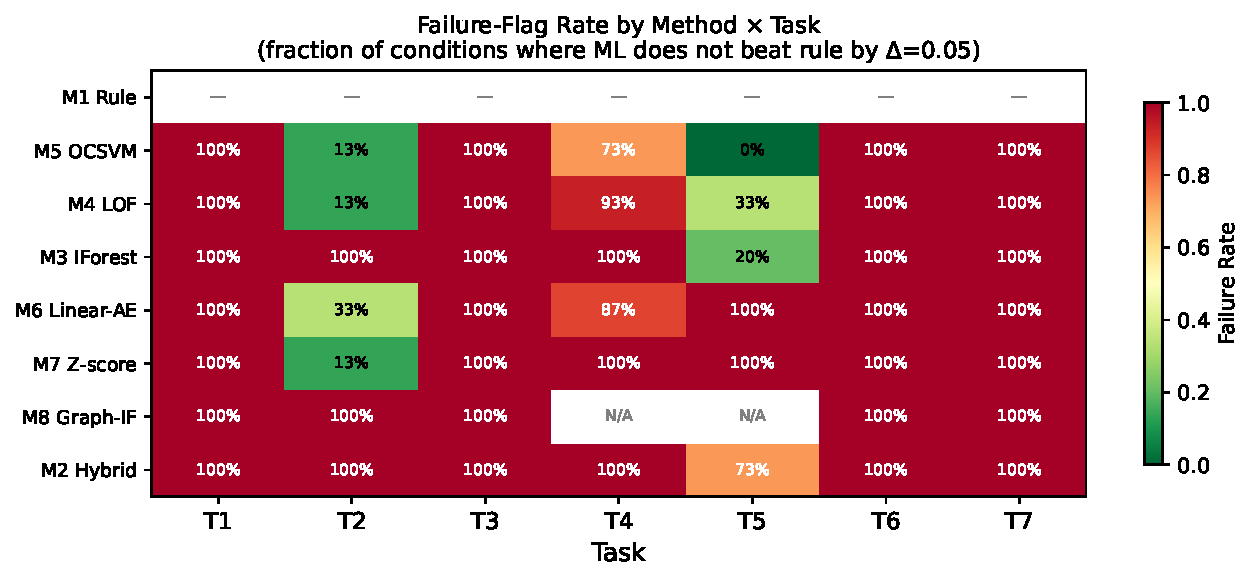
\includegraphics[width=\columnwidth]{figures/fig2_failure_heatmap.pdf}
  \caption{Failure-flag rate heatmap (method $\times$ task). Red cells indicate
    flagged configurations, ML fails to improve on the rule baseline by the
    pre-registered $\Delta$=0.05 threshold (Eq.~\eqref{eq:failure}) in
    $\geq$2/3 seeds; white cells (M8, T4-T5) are not applicable.\\
    \textit{Alt text:} Heatmap of failure-flag rate for 8 methods (rows M1-M8)
    against 7 tasks (columns T1-T7), where each cell shows the percentage of 5
    conditions flagged. Most cells are red at 100\%; green 0\% cells appear where
    ML adds value (for example M5 OCSVM at T2 and T5), and M8 Graph-IF is marked
    N/A for T4 and T5.}
  \label{fig:failure_heatmap}
\end{figure}

\begin{figure}[t]
  \centering
  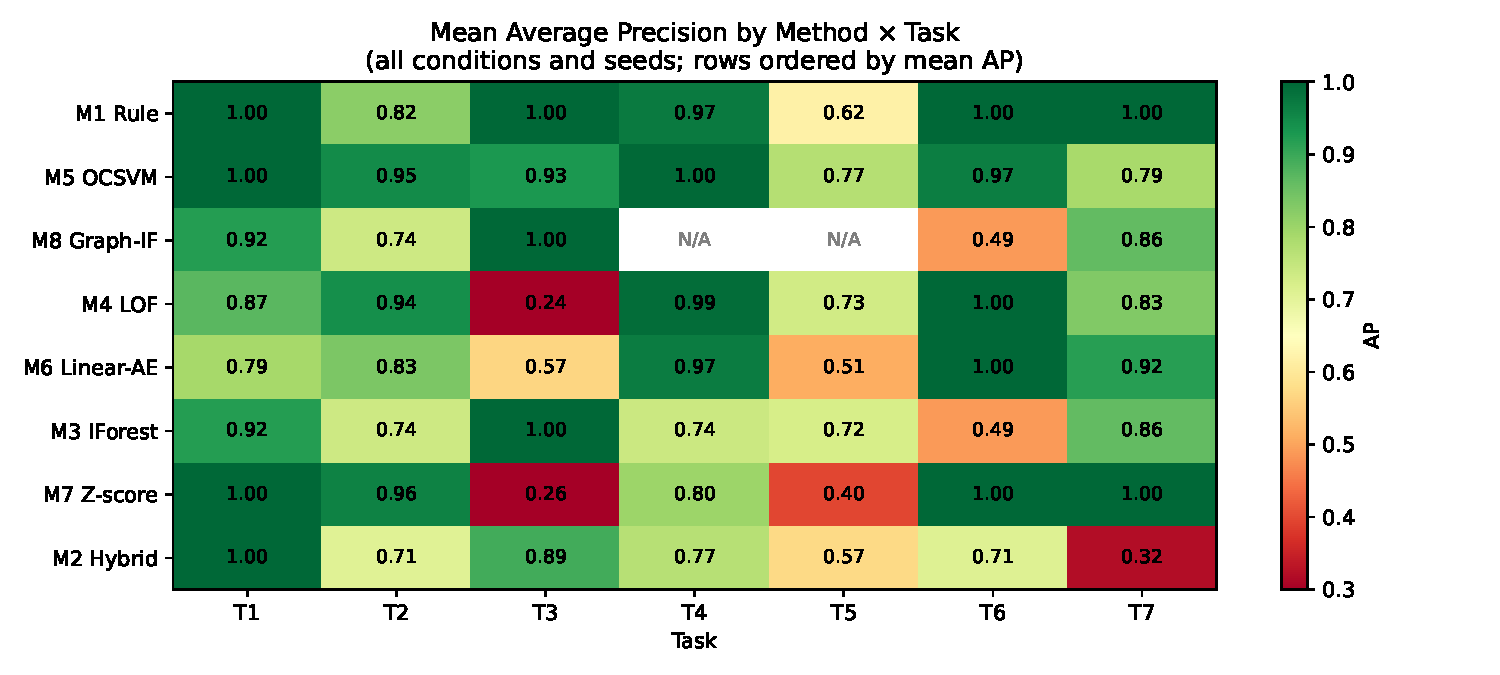
\includegraphics[width=\columnwidth]{figures/fig1_ap_heatmap.pdf}
  \caption{Condition-averaged AP heatmap (method $\times$ task). Higher values
    indicate better anomaly ranking. Rows are ordered by mean AP across all
    runs; M1 (rule baseline) anchors the top row.\\
    \textit{Alt text:} Heatmap of mean average precision for 8 methods (rows
    M1-M8) against 7 tasks (columns T1-T7), with values from about 0.24 to 1.00
    shaded red (low) to green (high). The M1 rule baseline row is highest overall;
    notable low cells include M4 LOF and M7 Z-score at T3, and M8 Graph-IF is N/A
    for T4 and T5.}
  \label{fig:ap_heatmap}
\end{figure}

\begin{figure*}[t]
  \centering
  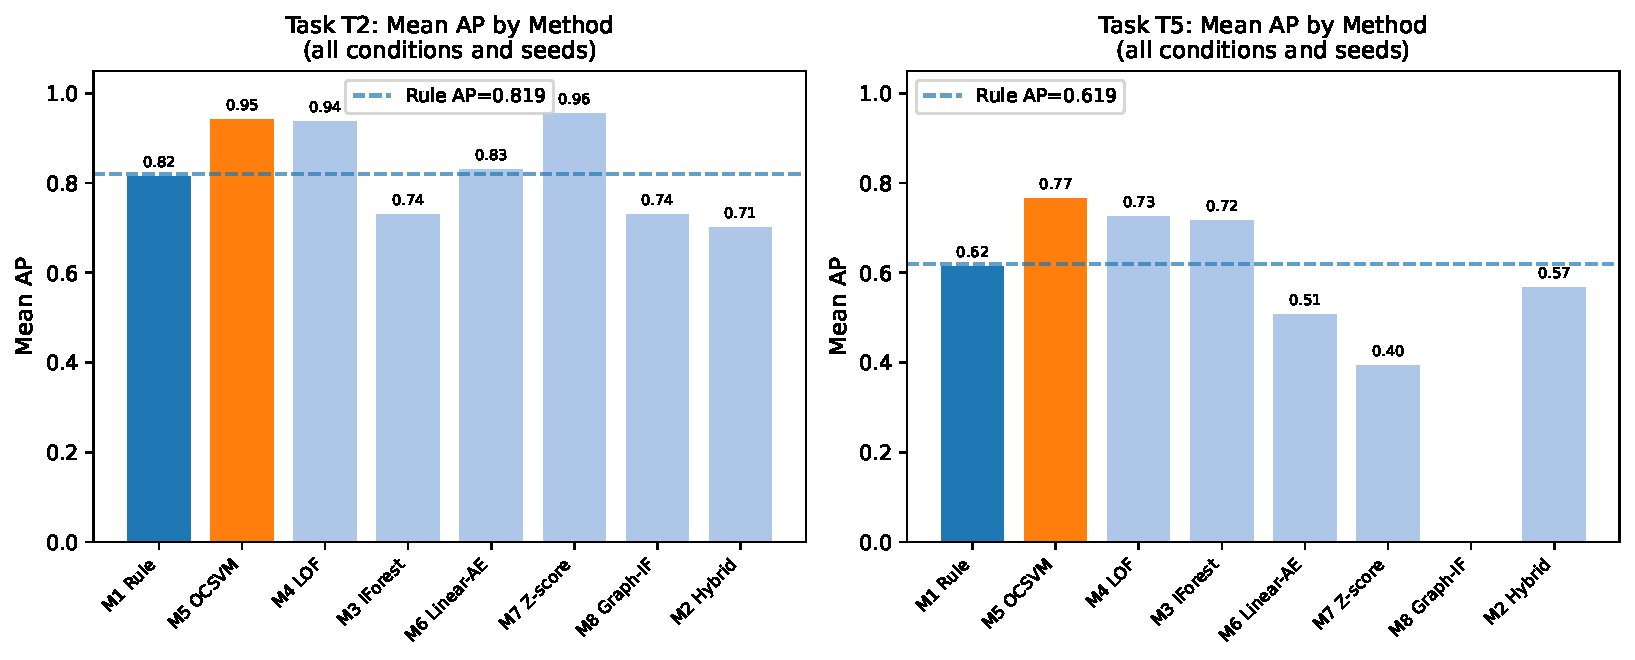
\includegraphics[width=\textwidth]{figures/fig4_t2_t5_ml_gain.pdf}
  \caption{AP by method for T2 (group membership drift) and T5
    (patch-vulnerability hygiene), averaged over all conditions and seeds, the
    two tasks where ML consistently adds value over the rule baseline.\\
    \textit{Alt text:} Two bar charts of mean average precision by method. For
    task T2 several methods exceed the dashed rule baseline of 0.819, led by
    M7 Z-score (0.96) and M5 OCSVM (0.95). For task T5 only M5 OCSVM (0.77) and
    M4 LOF (0.73) clearly beat the rule baseline of 0.619, while M7 Z-score (0.40)
    is the worst.}
  \label{fig:ml_gain}
\end{figure*}

\begin{figure*}[t]
  \centering
  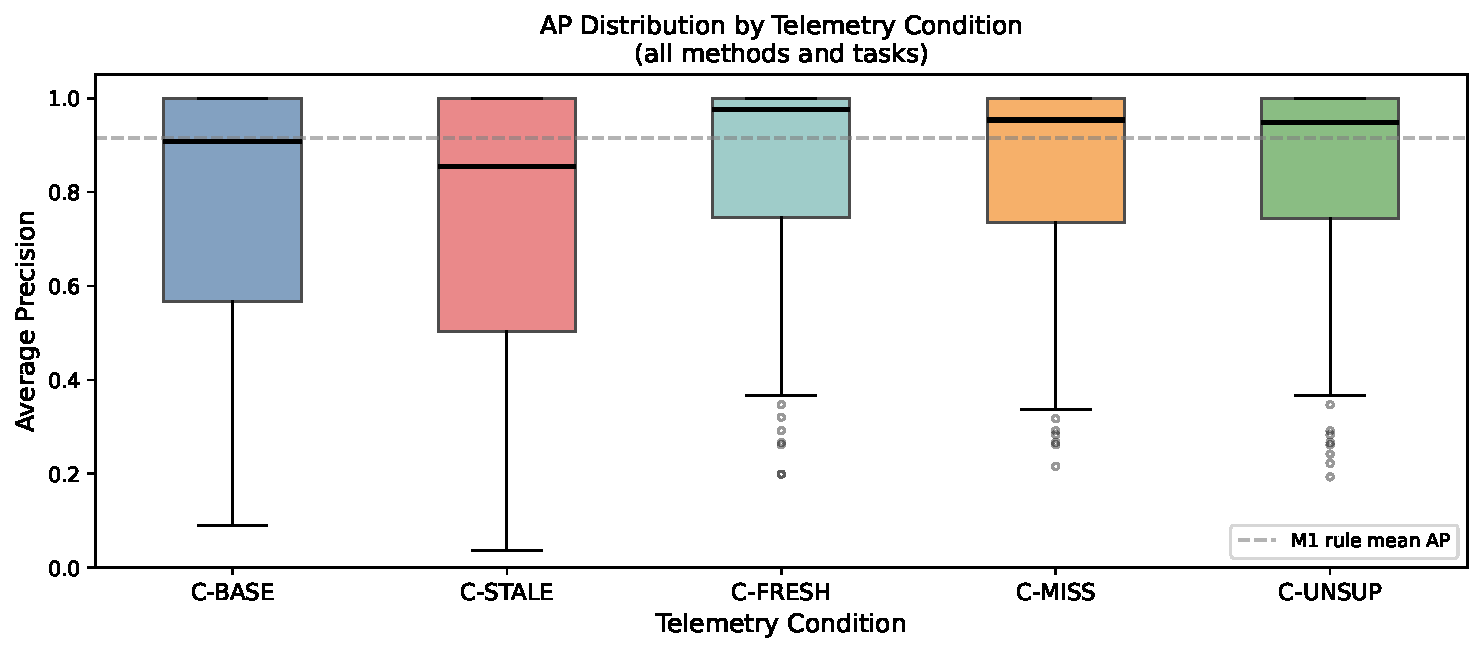
\includegraphics[width=\textwidth]{figures/fig3_ap_by_condition.pdf}
  \caption{AP distribution by telemetry condition (all tasks and methods). C-STALE
    has the lowest mean AP; C-FRESH has the highest.\\
    \textit{Alt text:} Box plots of average precision across five telemetry
    conditions (C-BASE, C-STALE, C-FRESH, C-MISS, C-UNSUP) over all methods and
    tasks. C-STALE shows the lowest and most spread-out distribution, while
    C-FRESH, C-MISS, and C-UNSUP have higher, tighter medians near the dashed
    M1 rule mean AP line, with several low outliers below 0.4.}
  \label{fig:ap_condition}
\end{figure*}
